\begin{center}
\begin{minipage}[t]{.46\linewidth}\vspace{0pt}\centering
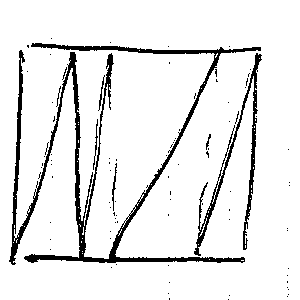
\includegraphics[width=\linewidth]{figures/gelfand-0154-p001416-interval-graph-original.png}\par\smallskip
{\footnotesize Оригинал рукописного рисунка: \texttt{GELFAND-P001416}}
\end{minipage}\hfill
\begin{minipage}[t]{.50\linewidth}\vspace{0pt}\centering
{\footnotesize Частичное воссоздание видимых штрихов}\par\smallskip
\resizebox{\linewidth}{!}{% Visible strokes only. Coordinate scale reproduces the sketch, not an exact map.
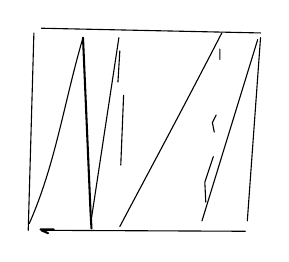
\begin{tikzpicture}[x=.012cm,y=-.012cm,line cap=round]
\draw (20,50)--(14,259) (28,45)--(260,50) (260,55)--(246,249)
 (31,259)--(244,260);
\draw (15,252) .. controls (43,189) and (52,123) .. (72,55);
\draw[line width=.75pt] (72,55)--(80,240)--(81,257);
\draw (81,246)--(110,55);
\draw (111,69)--(109,102) (115,116)--(112,190);
\draw (111,255) .. controls (140,200) and (171,143) .. (219,50);
\draw (198,249)--(257,57);
\draw (202,229)--(201,208)--(210,181) (211,155)--(209,145)--(213,137)
 (217,67)--(217,78);
% The thick bottom-left terminal trace is not interpreted as an arrow.
\draw[line width=.75pt] (27,258)--(41,258) (28,259)--(35,262);
\end{tikzpicture}
}
\end{minipage}
\end{center}
\noindent{\small\textit{Открытые соединения и короткие вертикальные штрихи остаются неустановленными после просмотра при 3×, 5× и 10×. Простые линии не задают стрелок, разрывов или дополнительных значений осей.}}
